\documentclass[a4paper,12pt]{report}
\usepackage[utf8]{inputenc}
\usepackage[french]{babel}
\usepackage[T1]{fontenc}
\usepackage{graphicx}
\usepackage{subcaption}
\usepackage[colorlinks,urlcolor=blue,citecolor=red]{hyperref} %hyperlinks
\usepackage{xcolor} %color text
\usepackage[amsthm]{ntheorem} %theorems and co.
\usepackage{amsmath} %mathematical symbols
\usepackage{amssymb} %squares in itemize
\usepackage[page,toc,titletoc,title]{appendix} %appendices
\usepackage[nottoc,notlot,notlof]{tocbibind} %bind the table of contents to the bibligoraphy
\usepackage{silence} %silencing warnings
\WarningFilter{latex}{Text page}

%Defining custom commands for relational model
\newcommand{\attr}[1]{\emph{#1}}
\newcommand{\texit}[1]{\#\textsl{#1}}

%Redefining the appendices name to "Annexes" in toc and removing "Annexe" from appendice title
\renewcommand{\appendixtocname}{Annexes}
\appendixtitletocoff

%Redefining the appendices name to "Annexes" in the report
\renewcommand{\appendixpagename}{Annexes}

%Defining a new command for the horizontal lines
\newcommand{\HRule}{\rule{\linewidth}{0.5mm}}

%Defining custom environments
\theoremstyle{break}
\newtheorem*{userStory}{User Story}

\theoremstyle{break}
\newtheorem*{definition}{Définition}

\theoremstyle{break}
\newtheorem*{property}{Propriété}

\theoremstyle{break}
\newtheorem*{constraint}{Règle}

\theoremstyle{definition}
\newtheorem*{example}{Exemple}

\theoremstyle{remark}
\newtheorem*{remark}{\textbf{Remarque}}

\begin{document}
\pagenumbering{roman}
%----------------------------------------------------------------------------------------
%   TITLE PAGE
%----------------------------------------------------------------------------------------
\begin{titlepage}
\centering
%----------------------------------------------------------------------------------------
%   LOGOS SECTION
%----------------------------------------------------------------------------------------

\includegraphics[scale=0.5]{images/umLogo.png} %Université de Montpellier Logo
\hspace{\fill}

\includegraphics[scale=0.25]{images/fdsLogo.jpg} %Faculté de Sciences Logo
\hspace{\fill}

\includegraphics[scale=0.25]{images/lirmmLogo.png}~\\[2cm] %LIRMM Logo
%----------------------------------------------------------------------------------------
%   HEADING SECTIONS
%----------------------------------------------------------------------------------------
\textsc{\LARGE L3 CMI Informatique}\\[0.5cm]
\textsc{\Large \textbf{HLIN601} -- TERL3}\\[0.25cm]
\textsc{\Large \texttt{CourtCircuit}}\\[2cm]
%----------------------------------------------------------------------------------------
%   TITLE SECTION
%----------------------------------------------------------------------------------------
\HRule \\[0.4cm]
{\huge \bfseries RAPPORT \#$2$}\\[0.1cm]
\HRule \\[2cm]
%----------------------------------------------------------------------------------------
%   STUDENTS SECTION
%----------------------------------------------------------------------------------------
\begin{minipage}{0.5\textwidth}
\centering \large
\textbf{Bachar \textsc{Rima}}\\
\textbf{Othmane \textsc{Farajallah}}\\
\textbf{Wissem \textsc{Soussi}}
\end{minipage} \\[2cm]
%----------------------------------------------------------------------------------------
%   SUPERVISORS SECTION
%----------------------------------------------------------------------------------------
\begin{minipage}[b]{0.5\textwidth}
\begin{flushleft} \large
\emph{Responsable CMI Informatique :} \\
Anne-Elisabeth \textsc{Baert} \\
\end{flushleft}
\end{minipage}
~
\begin{minipage}[b]{0.4\textwidth}
\begin{flushright} \large
\emph{Encadrant :}\\
Eric \textsc{Bourreau}
\end{flushright}
\end{minipage}\\[1.5cm]
%----------------------------------------------------------------------------------------
%   DATE SECTION
%----------------------------------------------------------------------------------------
{\large 5 mai 2018}\\[1cm]
\hspace{\fill}
\vfill % Fill the rest of the page with whitespace
\end{titlepage}
%----------------------------------------------------------------------------------------
%   TABLE OF CONTENTS
%----------------------------------------------------------------------------------------
{
  \hypersetup{linkcolor=black}
  \tableofcontents
  \setcounter{page}{3}
}
%----------------------------------------------------------------------------------------
%   REMERCIEMENTS
%----------------------------------------------------------------------------------------
\chapter*{Remerciements}
Nous tenons à remercier toutes les personnes ayant contribué de près ou de loin à la réussite de ce projet, en donnant des conseils ou en répondant à nos questionnements.

  Nous souhaitons également remercier en particulier M. Eric \textit{Bourreau} pour l'ensemble de ses efforts au cours de cette année, sachant répondre à l'ensemble de nos interrogations et également pour nous avoir donné l'opportunité de rencontrer des professionnels qui ont pu nous exposer leurs besoins ainsi qu'attentes envers notre projet en tant qu'utilisateurs potentiels.

%----------------------------------------------------------------------------------------
%   INTRODUCTION
%----------------------------------------------------------------------------------------
\chapter{Introduction}
\pagenumbering{arabic}
\setcounter{page}{1}
%----------------------------------------------------------------------------------------
%   CONTEXTE DU PROJET
%----------------------------------------------------------------------------------------
\section{Contexte du projet}
Dans ce rapport, nous nous consacrons à la description détaillée de la phase d'implémentation du projet intitulé \texttt{CourCircuit}\footnote{précédemment nommé \textbf{LaRuche}} effectué au sein du \textbf{LIRMM} (\textbf{L}aboratoire d'\textbf{I}nformatique, de \textbf{R}obotique et de \textbf{M}icroélectronique de \textbf{M}ontpellier) dans le cadre du module \textbf{HLIN601 -- TER} de la $3$\ieme{} année de licence en informatique \textbf{CMI} (\textbf{C}ursus \textbf{M}aster \textbf{I}ngénierie).

Le projet se déroule sous l'encadrement de Mme Anne-Elisabeth Baert, enseignante/chercheuse au sein du LIRMM dans l'équipe \textbf{MAORE} (\textbf{M}éthodes \textbf{A}lgorithmes pour l'\textbf{O}rdonnancement et les \textbf{Ré}seaux), en tant que responsable de la formation CMI informatique et M. Eric Bourreau, enseignant/chercheur au sein du LIRMM dans la même équipe \textbf{MAORE}, en tant que responsable pédagogique et encadrant du projet.

Le sujet du projet consiste à créer un site web représentant une interface de communication entre fournisseurs de produits locaux et leurs clients. Il est inspiré du site \og \href{https://laruchequiditoui.fr/fr}{La Ruche Qui Dit Oui} \fg traitant les mêmes problématiques, cependant adoptant une approche différente, surtout au niveau de la logistique et de l'architecture du site, afin de fournir une gestion plus optimisée des interactions directes entre clients et fournisseurs.

Nous commencerons ce rapport en faisant un récapitulatif du contexte du projet, des problématiques traitées, de la méthodologie et des outils de conception. De plus, nous proposerons une courte description des outils d'implémentation choisis. Après, nous procéderons à la description détaillée de ces outils et à tout en présentant les résultats obtenus. Enfin, nous conclurons en discutant les difficultés survenues lors du développement et les perspectives du projet.
%----------------------------------------------------------------------------------------
%   PROBLÈME, MÉTHODOLOGIE, OUTILS ET PLANNING
%----------------------------------------------------------------------------------------
\chapter{Problème, Méthodologie, et Outils}
%----------------------------------------------------------------------------------------
%   PROBLÈME
%----------------------------------------------------------------------------------------
\section{Problème}
Les consommateurs cherchent de \textit{plus en plus} à acheter des produits frais minimisant les étapes de \textit{processing}, alors que les producteurs cherchent à se libérer des centres d’achat et des intermédiaires de distribution.

Dans l’esprit du site francais \href{https://laruchequiditoui.fr/fr}{LaRucheQuiDitOui}, on souhaite implémenter une interface sous forme d'un \textbf{site web} d'\textit{e-commerce} permettant aux producteurs de vendre des sélections diversifiées de produits aux consommateurs en se regroupant dans des endroits précis de collecte.

Le site web offrira ainsi \textbf{tout ce dont il est nécessaire} aux consommateurs pour effectuer des commandes prépayées et précisera ensuite les points de collecte de produits les plus proches. D'autre part, il mettra à la disposition des fournisseurs la possibilité d'organiser ces points, de gérer la mise à jour des stocks et la mise en vente/prise de commandes par les clients, en se basant sur des algorithmes d'optimisation se portant aussi bien sur la gestion de la logistique, la préparation/facturation des commandes, que sur la redistribution/partage des produits entre les différents fournisseurs voisins.
%----------------------------------------------------------------------------------------
%   MÉTHODOLOGIE
%----------------------------------------------------------------------------------------
\section{Méthodologie}
Dans le but d'assurer une bonne gestion des ressources et d'offrir le plus de fonctionnalités possibles aux utilisateurs, en les implémentant itérativement dans des versions fonctionnelles et testées du site, nous avons opté pour une approche basée sur les \textbf{méthodes agiles} de développement, en particulier sur \textbf{XP}\footnote{\textit{eXtreme Programming}}.

En effet, la méthodologie de développement proposée par les méthodes agiles étant de plus en plus prépondérante en génie logiciel, nous avons décidé de l'utiliser pour la modélisation et l'implémentation de notre site web afin d'assurer le plus d'extensibilité et de flexibilité possibles.
%----------------------------------------------------------------------------------------
%   OUTILS DE CONCEPTION
%----------------------------------------------------------------------------------------
\section{Outils de conception}
Pour garantir une bonne modélisation du projet, en cohérence avec l'approche de la méthodologie discutée précédemment, nous avons explicité les spécifications fonctionnelles et organisationnelles de notre projet en se servant des outils suivants :
\begin{description}
  \item[\textit{user stories}]{des requis fournis par les utilisateurs décrivant en langage naturel les fonctionnalités qu'ils souhaitent avoir dans le site.}
  \item[diagrammes de cas d'usage]{des diagrammes dynamiques, souvent utilisés en \textbf{UML} pour décrire en haut niveau les fonctionnalités d'un système, en se servant de notions telles que \textbf{acteurs}, \textbf{cas d'usage}, \textbf{systèmes} et les \textbf{relations} entre chacune de ces entités.}
  \item[modèle EA]{un modèle \textbf{conceptuel} utilisé pour décrire les entités du projet ainsi que les associations décrivant leurs relations et comportements.}
  \item[schéma de base de données]{schéma en modèle \textbf{relationnel} composé des schémas des relations et des contraintes d'intégrité sur l'ensemble des relations, traduit généralement à partir du \textbf{modèle EA} et servant comme \textbf{modèle logique} lors de l'implémentation de la \textbf{base de données}.}
  \item[\textit{mockup storyboard}]{document de haut niveau offrant un moyen pour schématiser l'utilisation d'un projet, en positionant les différents éléments le composant, sans rentrer dans les détails de leur fonctionnement.}
\end{description}
%----------------------------------------------------------------------------------------
%   OUTILS D'IMPLÉMENTATION
%----------------------------------------------------------------------------------------
\section{Outils d'implémentation}
Afin de réaliser les impératifs de la partie conception du projet, nous avons prévu, pendant la partie de modélisation, d'utiliser principalement \textit{React.js}, \textit{JQuery}, \textit{Boostrap}, \textit{PHP} et \textit{MySQL}, ainsi que d'autres \textbf{API} pour l'implémentation de certaines parties du projet. Toutefois, après avoir compléter notre soutenance et suite à des recherches supplémentaires, nous avons décidé d'abandonner quelques technologies et de les remplacer par d'autres plus pertinentes afin d'obtenir un écosystème de travail plus cohérent et plus efficace.

Ce choix fût alimenté par plusieurs facteurs que nous discuterons plus en détail dans le chapitre \ref{chap:implementation_resultats} de ce rapport. Pour cette section, nous nous contentons simplement de fournir une courte description de l'ensemble de l'écosystème qui, en l'occurrence, est composé de :

\subsubsection{\textit{Front-end}}
\begin{description}
  \item [React.js :] une bibliothèque \textbf{JavaScript} créée par \textit{Facebook} et sortie en $2013$ pour la création des interfaces graphiques.
  \item [JSX :] (\textit{JavaScript XML}) une extension syntaxique du \textbf{JavaScript} permettant de simplifier la création des composants \textit{React} à travers une syntaxe à la \textbf{XML}.
  \item [Bootstrap :] un \textit{framework} \textbf{CSS} permettant la gestion du \textit{responsive web} du site.
\end{description}

\subsubsection{\textit{Back-end}}
\begin{description}
  \item [Node.js :] un environnement d'exécution \textbf{JavaScript} côté serveur gratuit et \textit{open-source} utilisant le moteur \textbf{JavaScript V8} de \textit{Google Chrome}.
  \item [Express :] un framework gratuit et \textit{open-source} pour construire des applications web et des \textbf{API}s sur \textbf{Node.js}.
  \item [MariaDB :] un serveur de base de données gratuit et \textit{open-source} remplaçant \textbf{MySQL} tout en restant compatible avec ce dernier.
\end{description}

Par conséquent, l'architecture des technologies choisies pour l'implémentation de notre projet est illustrée dans la figure \ref{fig:website_architecture}.

\begin{figure}[!ht]
  \centering
  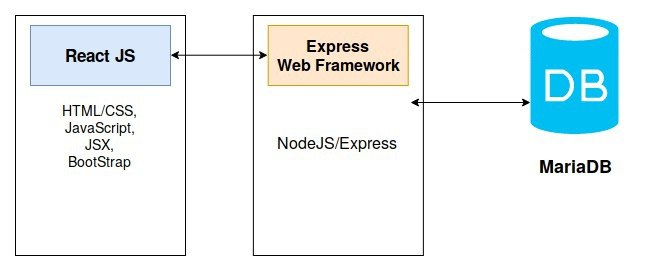
\includegraphics[scale=0.5]{images/website_architecture.jpeg}
  \caption{L'architecture des technologies utilisées en CourtCircuit}
  \label{fig:website_architecture}
\end{figure}

\newpage

\subsubsection{Editeur de texte}
\noindent
Pour la rédaction du code de notre projet, nous avons choisi unanimement d'utiliser l'éditeur de texte gratuit, \textit{open-source} et multiplateforme \textbf{Atom} pour son architecture basée sur \textbf{Node.js}. En effet, cette architecture permet de personnaliser son utilisation et de le rendre plus souple via des modules téléchargeables par le biais de son gestionnaire de packages \textbf{APM} (\textit{Atom Package Manager}).
%----------------------------------------------------------------------------------------
%   IMPLÉMENTATION
%----------------------------------------------------------------------------------------
\chapter{Implémentation et Résultats}
\label{chap:implementation_resultats}
%----------------------------------------------------------------------------------------
%   APPLICATION WEB MONOPAGE
%----------------------------------------------------------------------------------------
\section{Application web monopage}
Avant l'introduction d'\textbf{AJAX}\footnote{\textit{Asynchronous JavaScript and XML}}, un application web classique était composée de plusieurs fichiers \textbf{HTML} incorporant la structure de ses pages, avec des feuilles de styles \textbf{CSS} pour la mise-en-forme et des scripts \textbf{JavaScript} \textit{front-end} classiques manipulant le \textbf{DOM} pour rendre les pages dynamiques via l'\textbf{API DOM} ou des bibliothèques facilitant cette manipulation telles que \textbf{JQuery}.

Après l'introduction d'\textbf{AJAX}, qui a permis de changer une page dynamiquement sans besoin de la recharger, une nouvelle structuration des applications webs a commencé à émerger, notamment la structuration monopage (\textbf{SPA} ou \textit{Single Page Application}).

Une application web est dite monopage quand elle est composée d'une unique page HTML associée à des ressources Javascript et CSS permettant de changer son contenu dynamiquement. Cette action met en place un effet illusoire de transition entre pages bien qu'il s'agit en réalité d'une seule page rechargée.

Avec une application web classique, le rôle d'un navigateur est, grosso modo, de transmettre au serveur les actions et données saisies par le client et d'afficher les pages HTML générées par le serveur au retour.

Avec une application web monopage, le rôle du navigateur devient plus important, consistant à interagir avec les actions de l'utilisateur et faire une première validation des informations saisies. Le serveur sera libéré ainsi pour les traitements des données reçues et à transmettre tout en effectuant une seconde validation des informations pour assurer leur intégrité.

Une application web monopage devient alors une véritable \og application \fg qui tourne dans le navigateur du client pour améliorer son expérience et
éviter de surcharger le serveur avec la génération de pages entières après chaque requête envoyée.

Pour ces raisons nous avons ainsi décidé d'adopter une modélisation monopage pour notre application web tout en expérimentant avec les technologies associées permettant sa mise en \oe{}uvre.
%----------------------------------------------------------------------------------------
%   FRONT-END
%----------------------------------------------------------------------------------------
\section{Front-end}
Pour la partie \textit{front-end}, nous avons décidé d'utiliser \textbf{React.js}/\textbf{JSX} pour les interfaces graphiques et \textbf{Bootstrap} pour le \textit{responsive web}. Nous détaillerons les raisons pour ce choix et l'utilisation de ces outils dans les sections suivantes.
%----------------------------------------------------------------------------------------
%   REACT-JS
%----------------------------------------------------------------------------------------
\subsection{React.js et JSX}
\textbf{React} est une bibliothèque \textbf{JavaScript} libre développée par \textbf{Facebook} en $2013$. Elle permet de créer des interfaces hautement personnalisables et interactives pour des applications monopages.

Nous avons choisi \textbf{React} au vu des nombreux points forts que possède le paradigme de la programmation réactive. En effet c’est un style de programmation qui se prête très bien aux interfaces graphiques puisqu’il est généralement possible de définir une représentation statique et plusieurs états de son interface d'une manière asynchrone.

D’autre part, \textbf{React} est connue pour sa performance. Les applications développées en \textbf{React} peuvent gérer des mises à jour complexes tout en restant rapides et réactives. \textbf{React} est aussi modulaire; au lieu d’écrire de gros fichiers de code denses on peut écrire beaucoup de petits fichiers réutilisables.

\subsubsection{Le DOM virtuel}
Une page \textbf{HTML} classique est représentée sous forme d'un arbre \textbf{DOM} dans le navigateur. Quand un changement est appliqué à un ou plusieurs éléments préalablement chargés dans le \textbf{DOM}, le navigateur doit effectuer de nombreuses opérations impliquant un coût mémoire important, notamment en rechargeant et repositionnant l’ensemble des n\oe{}uds.

Pour minimiser ce coût, \textbf{React} agit sur l’affichage dans le navigateur en utilisant un système de \textbf{DOM virtuel}. Ce dernier est une représentation du \textbf{DOM} en \textbf{JavaScript} qui est plus rapide en écriture.

Quand une modification est appliquée, \textbf{React} calcule les changements à opérer et recharge uniquement les parties du \textbf{DOM} impactées. Les opérations coûteuses sont ainsi évitées. Cette approche permet ainsi de fournir des performances exceptionnelles.

\subsubsection{La modularité}
\begin{figure}[!ht]
  \centering
  
\includegraphics[scale=0.35]{images/header_navbar_component.png}
  \caption{Barre de navigation du site fait avec \textbf{Bootstrap} et représentant un composant de type \textit{Component}}
  \label{fig:header_navbar_component}
\end{figure}

Une application \textbf{React} peut être représentée par un ensemble de composants imbriqués les uns dans les autres. L’intérêt majeur de cette architecture est qu’elle permet la réutilisabilité de \og morceaux de code \fg pour économiser son écriture et améliorer sa lisibilité mais également afin de faciliter la maintenance.

Cette fonctionnalité est un gage de productivité permettant de facilement définir et manipuler l’ensemble des éléments constituant notre interface graphique.
Pour implémenter ce concept de composants, nous avons adopté une organisation inspirée du patron de conception \textit{Container Component}. Dans cette organisation, nous avons séparé nos composants en deux catégories :

\begin{enumerate}
  \item une partie \textit{Components} incluant les éléments qui s’occupent uniquement de présenter les informations au \textbf{DOM}. Ce sont donc des éléments indépendants prenant en charge l’aspect visuel de notre application, comme par exemple les éléments \textit{header, footer, navigation bar} (cf. Figure \ref{fig:header_navbar_component})
  \item une partie \textit{Containers} qui inclut les éléments responsables de gérer les changements de \textit{state} en correspondant chaque état avec un comportement particulier. Ce sont donc des composants de haut niveau qui fournissent aux \textit{Components} les données qu’il faut afficher.
\end{enumerate}

Cette séparation permet d'optimiser la réutilisabilité des composants, et de faciliter la relecture du code en les distinguant selon leurs rôles. Quelques éléments de l'interface graphique sont consultables dans les annexes de ce rapport.

\subsubsection{JSX : \textit{JavaScript XML}}
\textbf{React} peut s’écrire avec une syntaxe \textbf{JavaScript pure}. Toutefois, ce processus devient fort répétitif et illisible. Pour gagner en lisibilité et économie d'écriture, \textbf{JSX} a été introduit comme extension syntaxique du \textbf{JavaScript}, d'où notre choix de l'utiliser dans notre projet.

\textbf{JSX} rend le code beaucoup plus souple à lire et écrire, et donc facilite la compréhension du code et le rend plus déclarative. Cependant, \textbf{JSX} ne pouvant être interprété par le navigateur, \textbf{Babel} a proposé un \textit{preset} permettant de transpiler le code \textbf{JSX} en code \textbf{JavaScript} classique et interprétable par le navigateur.
%----------------------------------------------------------------------------------------
%   BOOTSTRAP
%----------------------------------------------------------------------------------------
\subsection{Bootstrap et Font Awesome}
\textbf{Bootstrap} est un \textit{framework open-source} et gratuit pour le développement \textit{front-end} d'un site web. Il est pricipalement un \textit{framework} \textbf{CSS} bien qu'il embarque aussi des composants \textbf{JavaScript} et \textbf{HTML}.

En utilisant un système de grille pour gérer la mise en forme d'une page, \textbf{Bootstrap} est capable d'adapter dynamiquement les éléments d'une page par rapport à la taille de la fenêtre du navigateur, permettant ainsi d'avoir un site web \textit{responsive} utilisable sur toute sorte d'écrans (\textit{smartphone, tablet, moniteur, téléviseur, $\dots$}).

D'autre part, \textbf{Bootstrap} offre un ensemble de classes \textbf{CSS}, des éléments prêts à l'usage (\textit{boutons, formulaires, accordéons, menus de navigation, $\dots$}), et des animations implémentées en \textbf{JQuery}, tout en rendant possible leur personnalisation. Ceci permet alors un développement rapide d'une application web avec peu de lignes de code.

\begin{figure}[!ht]
  \centering
  
\includegraphics[scale=0.35]{images/footer.png}
  \caption{\textit{Footer} du site fait avec les icônes de \textbf{Font Awesome}}
  \label{fig:footer_font_awesome}
\end{figure}

Dans notre projet, nous avons alors eu recours à \textbf{Bootstrap} pour éviter la redéfinition de l'aspect esthétique de chaque élément HTML à partir du zéro.

D'autre part, nous nous sommes servis aussi des outils fournis par \textbf{Font Awesome}. \textbf{Font Awesome} a été créé pour être utilisé avec \textbf{Bootstrap} en rendant les icônes utilisables en tant que polices pouvant subir des changement de styles via CSS, SASS et LESS.

Ainsi en se servant de ces deux technologies, chaque composante \textbf{React} du site a été esthétiquement personnalisée, par exemple :
\begin{itemize}
  \item le \textit{header} du site (cf. Figure \ref{fig:header_navbar_component}) contient une barre de navigation \textit{responsive} pouvant être pliée et dépliée ;
  \item le \textit{footer} du site (cf. Figure \ref{fig:footer_font_awesome}) contient des icônes fournis par \textbf{Font Awesome} comme liens vers d'autres pages.
\end{itemize}
%----------------------------------------------------------------------------------------
%   CHARTE GRAPHIQUE
%----------------------------------------------------------------------------------------
\subsection{Charte graphique}
\begin{figure}[!ht]
  \centering
  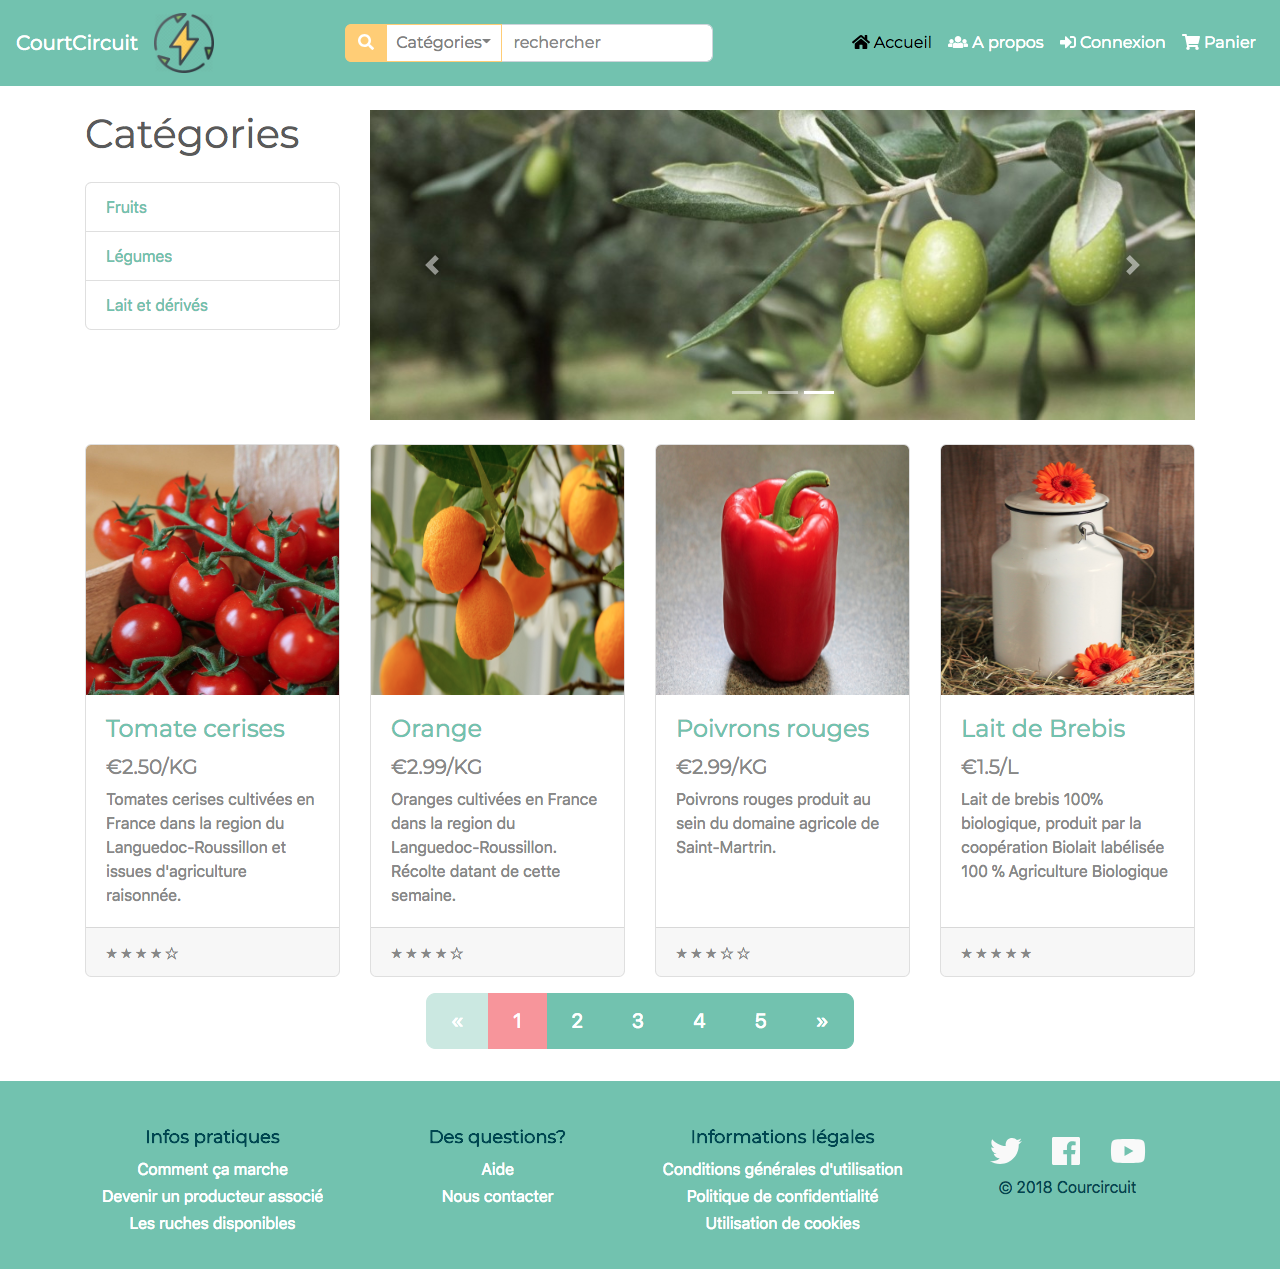
\includegraphics[scale=0.3]{images/accueil.png}
  \caption{Page d'accueil du site web}
  \label{fig:page_accueil}
\end{figure}

Le site web, étant principalement un site \textit{e-commerce} de fruits et de légumes\footnote{entre autres} (cf. Figure \ref{fig:page_accueil}), nous avons pensé à utiliser pour les éléments du site des couleurs telles que le vert et l'orange. Ces couleurs reflètent un aspect naturel et associe aux produits affichés la qualité de fraîcheur. De plus, les polices, couleurs et logos sont sombres et simples.
%----------------------------------------------------------------------------------------
%   BACK-END
%----------------------------------------------------------------------------------------
\section{Back-end}
Pour la partie \textit{back-end}, nous avons décidé d'utiliser \textbf{Node.js}/\textbf{Express.js} pour le serveur et \textbf{MariaDB} pour la base de données. Nous détaillerons les raisons pour ce choix et l'utilisation de ces outils dans les sections suivantes.
%----------------------------------------------------------------------------------------
%   NODE.JS
%----------------------------------------------------------------------------------------
\subsection{Node.js}
\begin{figure}[!ht]
  \centering
  
\includegraphics[scale=0.04]{images/nodejs_icon.png}
  \caption{le logo de \textbf{Node.js}}
\end{figure}

\textbf{Node.js} est un environnement d'exécution \textbf{JavaScript} côté serveur utilisant le moteur \textbf{JavaScript V8} de \textit{Google Chrome}. Il est libre, gratuit et doté d'une efficacité et d'une légèreté provenant de sa modélisation événementielle, monothread et non-bloquante et de son architecture modulaire. Sa facilité d'usage et son extensibilité est dûe aussi à son gestionnaire de paquets \textbf{NPM} (\textit{Node Package Manager}) considéré comme l'un des plus larges écosystèmes de librairies \textit{open-source} au monde.

\textbf{Node.js} est une technologie récente qui est de plus en plus utilisée, surtout en développement web avec les architectures \textbf{MERN} (\textit{MongoDB Express React Node}) et \textbf{MEAN} (\textit{MongoDB Express Angular Node}). Par suite, ceci nous a motivé à l'intégrer dans notre projet au vu de ses nombreuses avantages.

En premier, notre choix de \textbf{Node.js} découle du fait qu'il permet d'écrire du code \textbf{JavaScript} du côté serveur. Cette particularité nous a permis d'unifier la rédaction du code en un seul langage, pour les côtés client et serveur. En effet, l'unification du code a rendu possible à l'ensemble du groupe de participer au débogage du projet entier sans aucune restriction liée à la maîtrise d'un langage ou l'autre.

Outre l'unification du code, étant donné que nous aurons besoin de gérer un ensemble important de données dans le cadre de notre projet, l'aspect monothread et non-bloquant de \textbf{Node.js} assure une performance fluide que nous ne trouverons pas forcément avec d'autres technologies \textit{back-end}, utilisant généralement des modèles multi-processus ou multithread.

Enfin, \textbf{Node.js} est le choix par défaut pour une architecture utilisant \textbf{React.js}\footnote{bien que pas le seul}, ce qui nous a encouragé davantage à s'en servir.

Dans le cadre de notre projet, nous avons principalement utilisé \textbf{Node.js} pour la création d'une \textbf{API} côté serveur permettant d'interfacer avec la base de données. Ceci fût concrétisé par la création des objets pour les différentes entités manipulés (\textit{Client, Utilisateur, Produit, $\dots$}), en s'appuyant sur des concepts de la programmation orienté-objet. Par conséquent, nous avons pu factoriser le code pour éviter les redondances et  améliorer sa lisibilité lors de l'exécution des requêtes sur la base de données.

D'autre part, nous nous sommes également servi de \textbf{Node.js} pour l'utilisation du framework \textbf{Express} que nous détaillerons dans la section suivante.
%----------------------------------------------------------------------------------------
%   EXPRESS
%----------------------------------------------------------------------------------------
\subsection{Express}
\begin{figure}[!ht]
  \centering
  
\includegraphics[scale=0.4]{images/express_icon.png}
  \caption{Le logo de \textbf{Express}}
\end{figure}

\textbf{Express} est un framework minimaliste gratuit et \textit{open-source}, devenu standard pour construire des applications web et des \textbf{API}s côte serveur sur \textbf{Node.js}. Il s'appuie sur des concepts \textbf{MVC} (\textit{Model View Controller}) et offre plusieurs services notamment l'utilisation de moteurs de templates (\textit{EJS (Embedded JavaScript), Handlebars, et Jade}), l'utilisation de \textit{middleware}, la gestion des routes et des formulaires, $\dots$.

Dans le cadre de notre projet nous nous sommes principalement servi d'\textbf{Express} pour la gestion côté serveur des routes implémentées par \textbf{React} en implémentant les opérations \textbf{CRUD} (\textit{Create, Read, Update, Delete}) correspondantes.
%----------------------------------------------------------------------------------------
%   MARIADB
%----------------------------------------------------------------------------------------
\subsection{MariaBD}
\begin{figure}[!ht]
  \centering
  
\includegraphics[scale=0.4]{images/mariadb_icon.png}
  \caption{Le logo de \textbf{MariaDB}}
\end{figure}

En général, le serveur de base de données \textbf{MongoDB} est le choix par défaut pour une architecture incluant \textbf{React}, \textbf{Node.js} et \textbf{Express}. Ceci est dû principalement à sa modélisation \textbf{NoSQL} basée sur des documents au format \textbf{JSON} facilitant la récupération et le stockage des données à travers une technologie \textit{back-end} utilisant \textbf{JavaScript} telle que \textbf{Node.js}.

Toutefois, vu que nous avions déjà traduit notre \textbf{modèle EA} (cf. Figure \ref{fig:modele_EA}) en \textbf{modèle relationnel}, et vu que le serveur de la faculté qui nous a été attribué pour le déploiement de notre site n'hébérgeait pas un serveur \textbf{MongoDB} mais hébérgeait bien son contrepartie \textbf{MySQL}, nous avons opté pour un \textbf{SGBD} relationnel classique, notamment \textbf{MariaDB}.

\textbf{MariaDB} est un serveur de base de données gratuit et \textit{open-source}, assurant l'interopérabilité avec \textbf{MySQL}, qui fût introduit par les créateurs de \textbf{MySQL} suite à l'achat de ce dernier par \textbf{Oracle}. Il s'agit en réalité d'un fork communautaire de \textbf{MySQL} qui est mis à jour plus souvent que \textbf{MySQL}.

Pour toutes ces raisons, nous avons ainsi décidé d'adopter \textbf{MariaDB} comme \textbf{SGBD} de notre base de données.

Pour interfacer \textbf{Node.js} et \textbf{MariaDB} nous avons eu recours au \textit{package} \og \texttt{mysql} \fg que nous avions téléchargé via \texttt{npm}. Le package contient l'ensemble des fonctionnalités permettant de se connecter à la base de données et d'exécuter des requêtes \textbf{SQL} là-dessus.

\begin{figure}[!ht]
  \centering
  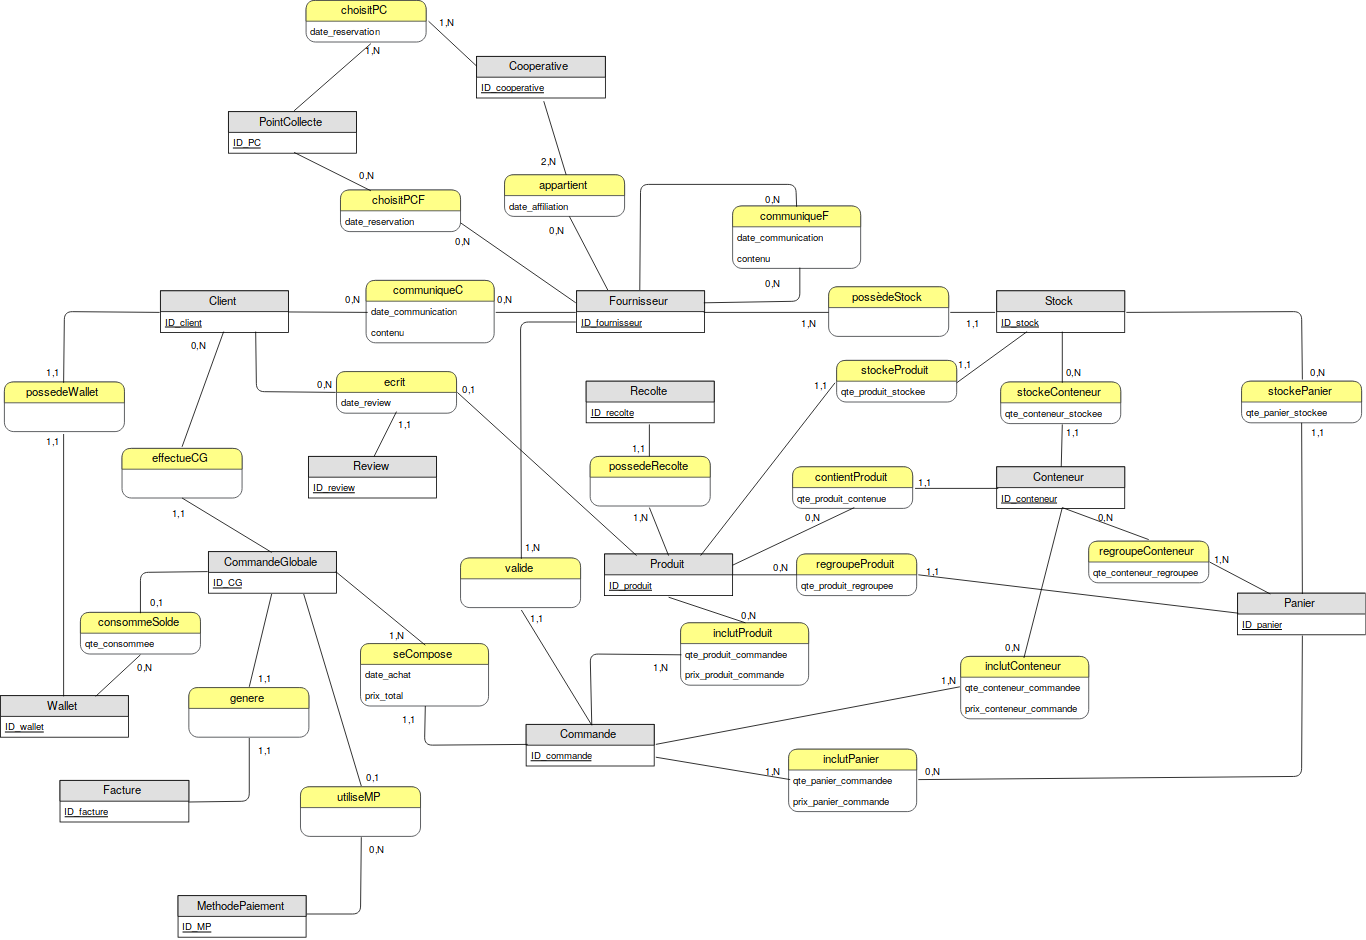
\includegraphics[scale=0.35]{images/er_model.png}
  \caption{Modèle Entité-Association}
  \label{fig:modele_EA}
\end{figure}

\newpage
%----------------------------------------------------------------------------------------
%   CONCLUSION
%----------------------------------------------------------------------------------------
\chapter{Conclusion}
%----------------------------------------------------------------------------------------
%   DIFFICULTÉS SURVENUES
%----------------------------------------------------------------------------------------
\section{Difficultés survenues}
Nous avons rencontré plusieurs difficultés pendant le développement du projet, notamment des difficultés liées à la maîtrise des outils nécessaires pour son développement, et que nous n'avons jamais utilisés auparavant (\textit{React, JSX, Express $\dots$}).

D'autre part, le temps que nous avions prévu d'accorder à la partie modélisation s'est révelé insuffisant. Nous avons donc été obligés d'y consacrer plus de temps pour avoir un résultat cohérent. Ceci a eu des répercussions négatives sur notre livrable final.

De plus, nous avons eu un souci avec le serveur d'hébergement du département informatique. En effet, le serveur hébérgea des versions anciennes de \textbf{Node} et \textbf{NPM} et nous n'avons pas accès à une base de données dediée à notre projet comme c'était indiqué sur l'espace projets du \textbf{SIF}. Ainsi, n'ayant pas les droits d'accès nécessaires pour rectifier ces problèmes, nous n'avons pas pu héberger notre site en ligne. Par conséquent, nous étions obligés de travailler sur notre application et de tester l'ensemble de ses fonctionnalités localement.
%----------------------------------------------------------------------------------------
%   PERSPECTIVES
%----------------------------------------------------------------------------------------
\section{Perspectives}
\label{sec:perspectives}
Outre les fonctionnalités que nous avons jugées essentielles au projet, nous avons pensé à ajouter des fonctionnalités supplémentaires une fois celles de base établies. En effet, plusieurs extensions sont possibles afin de proposer aux utilisateurs un choix plus diversifié et plus complet.

Dans ce cadre, nous avons prévu de donner aux clients la possibilité de régler des achats à l'aide d'une carte bancaire mais également à l'aide de services de paiements en ligne tels que Paypal. En addition, nous pourrions également internationaliser le site et son concept en proposant des versions
en plusieurs.

Enfin, nous nous sommes aperçus de plus en plus que le projet est devenu une source d'intérêt personnel, au point où nous souhaiterons fort probablement le poursuivre au niveau individuel au delà le cadre de ce module.
%----------------------------------------------------------------------------------------
%   APPORT PERSONNEL
%----------------------------------------------------------------------------------------
\section{Apports personnels}
Tout au long du projet, chaque difficulté rencontrée était une nouvelle expérience enrichissante. L'apprentissage de nouveaux concepts de programmation web et la maîtrise de nouvelles technologies associées, que nous n'avions guère manipulés au préalable, était un défi profondément apprécié. En particulier, nous avons eu la chance de profiter des richesses offertes par JavaScript dans différents contextes, ce qui a radicalement changé notre perception du langage.

Nous sommes convaincus que, jusqu'à présent, ce projet fût le plus intéressant, quoique le plus exigeant, parmi les projets auxquels nous avions participé. De plus, nous sommes bien ravis par les connaissances acquises qui se prouverons certainement utiles ultérieurement dans nos formations futures mais également dans nos démarches professionnelles.
%----------------------------------------------------------------------------------------
%   ANNEXES
%----------------------------------------------------------------------------------------
\begin{appendices}
\pagenumbering{roman}
\setcounter{page}{1}

\chapter{Snapshots du site}
Dans ce chapitre, nous illustrons quelques snapshots de notre application web.

\begin{figure}[!ht]
  \centering
  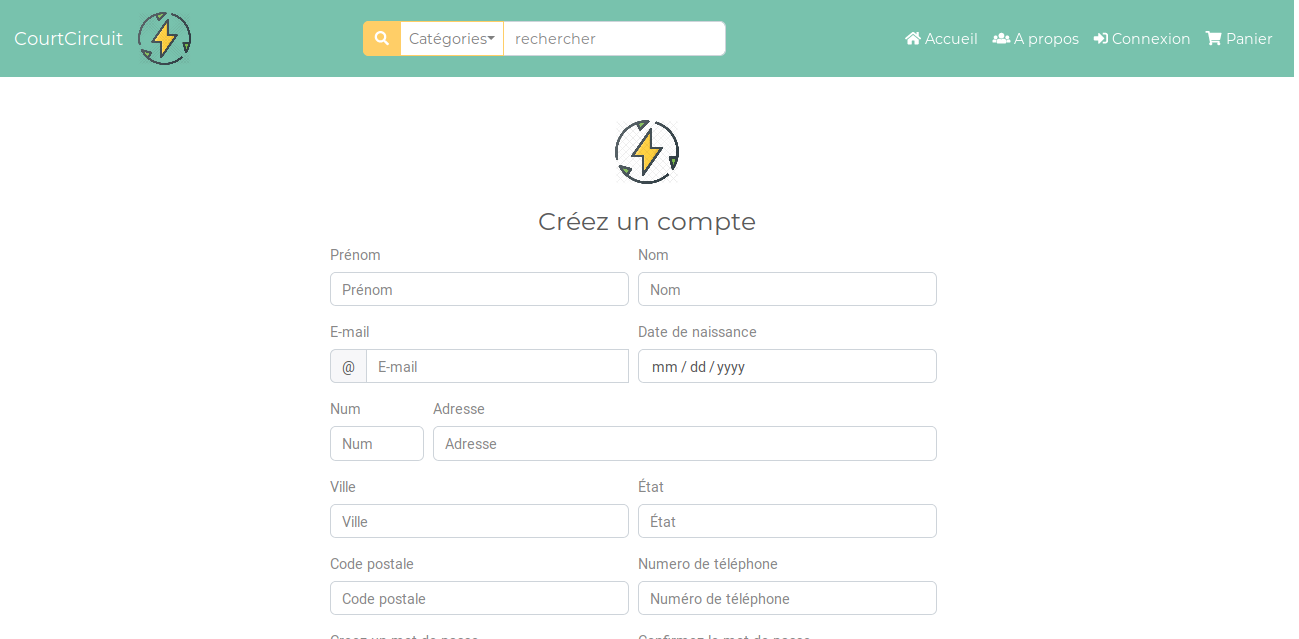
\includegraphics[scale=0.35]{images/signUp.png}
  \caption{La page d'inscription}
\end{figure}

\begin{figure}[!ht]
  \centering
  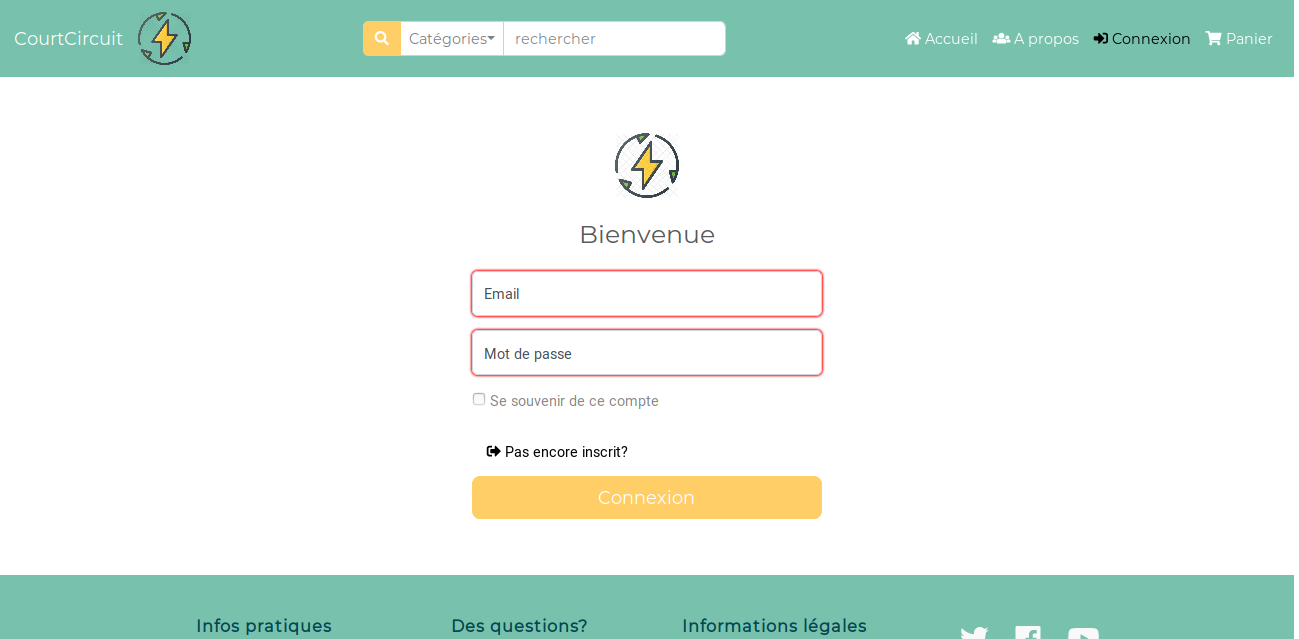
\includegraphics[scale=0.35]{images/signIn.png}
  \caption{La page de connexion}
\end{figure}

\begin{figure}[!ht]
  \centering
  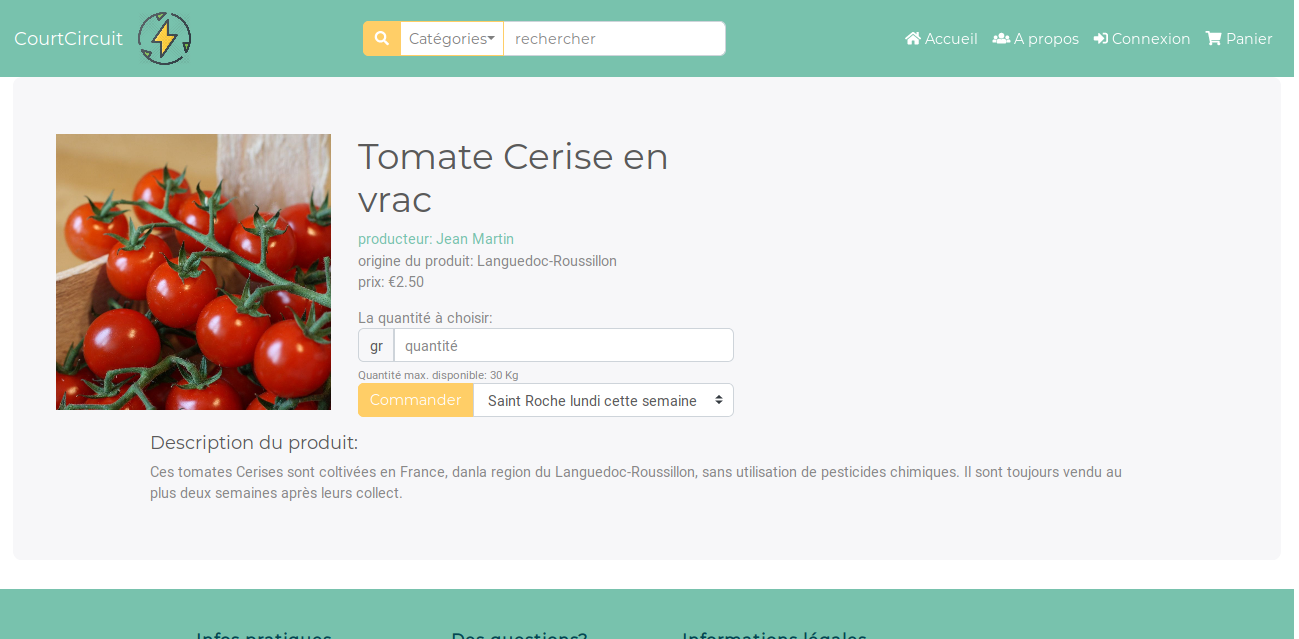
\includegraphics[scale=0.35]{images/produit.png}
  \caption{La page d'un produit}
\end{figure}

\begin{figure}[!ht]
  \centering
  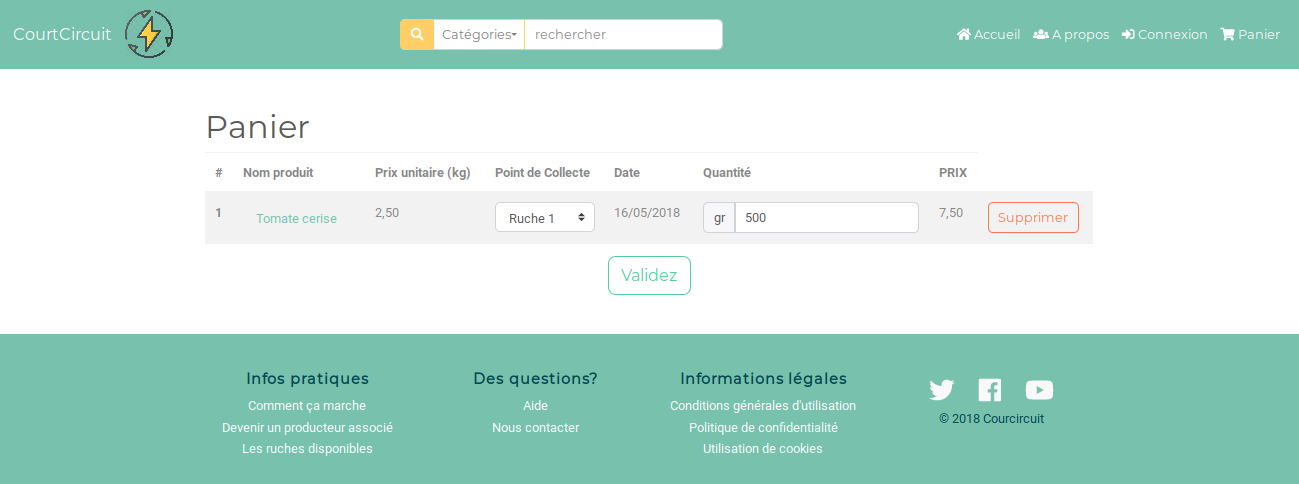
\includegraphics[scale=0.35]{images/cart.png}
  \caption{La page du chariot}
\end{figure}

\begin{figure}[!ht]
  \centering
  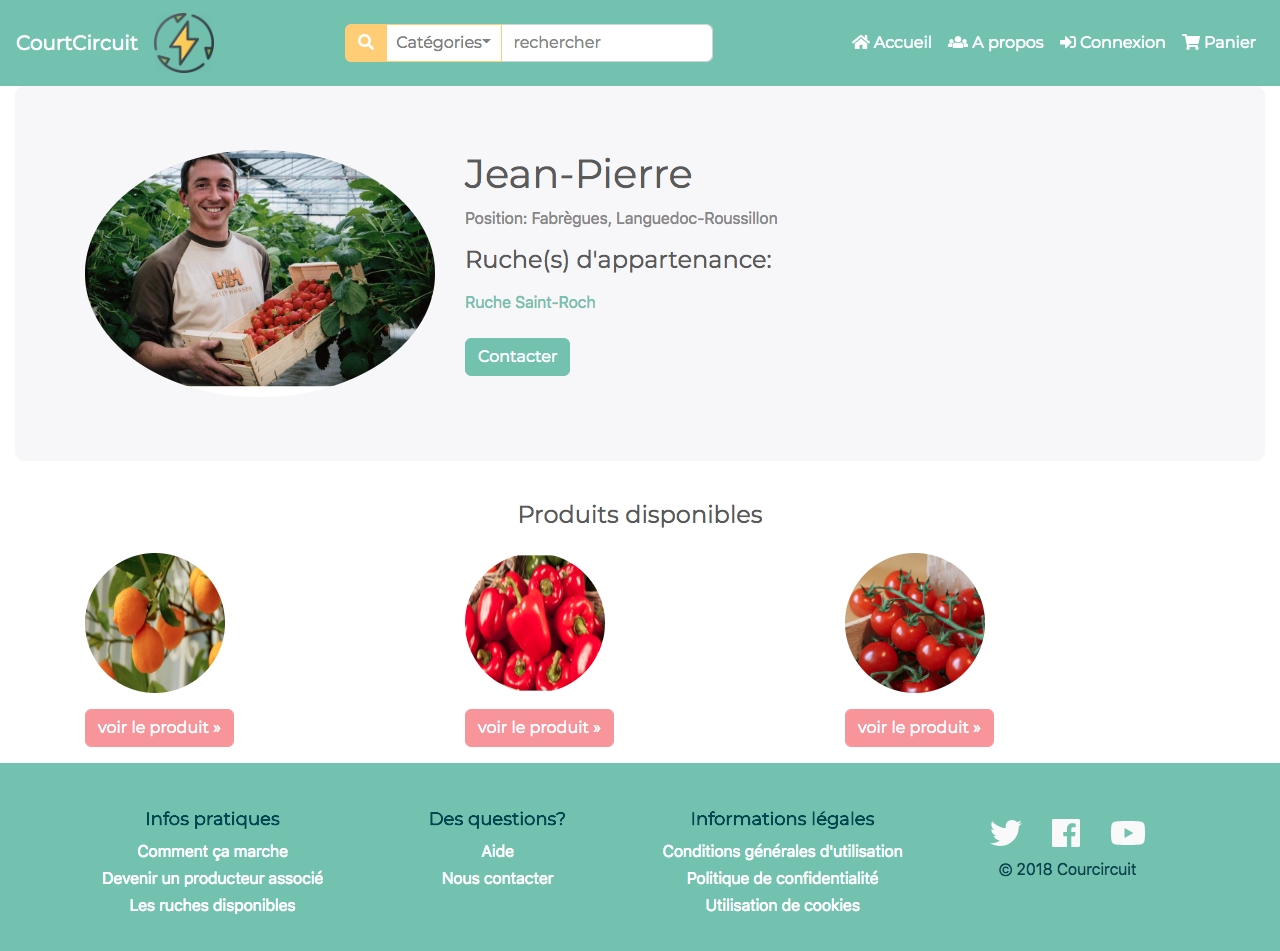
\includegraphics[scale=0.35]{images/vendeur.png}
  \caption{La page d'un vendeur}
\end{figure}
\end{appendices}
\end{document}
